%%%%%%%%%%%%%%%%%%%%%%%%%%%%%%%
%%%%%%%%%%%%%%%%%%%%%%%%%%%%%%%
\chapter{Introduction}
%%%%%%%%%%%%%%%%%%%%%%%%%%%%%%%
The use of twin models is a not a new idea. NASA build twin rockets for the Apollo missions, where one rocket went to the Moon and the other twin rocket stayed on Earth.
The twin model could be used as a reference object if something went wrong during the mission.  
The twin model concept has a lot of other usefully applications, not just for catastrophic scenarios with a failing space ship, but also for more ordinary applications such as conventional ships. Building a real twin ship as a reference object is of course not realistic. With data recorded onboard ships it is instead possible to build a ship digital twin (SDT), to serve the same purpose.
System identification methods of Ship Rigid Body Dynamics are presented in this thesis, which can be used as important sub-components in the SDTs. 

Ship dynamics is a branch of ship hydrodynamics which concerns the ship forces and motions when the ship is allowed to move and rotate in all directions. Seakeeping and Manoeuvring are the two major sub fields (see \autoref{fig:seakeeping_and_manoeuvring}), where Seakeeping studies the  behaviour of a ship in a seaway, under the influence of the external waves, currents and winds. Calm water conditions, lacking the external waves, are further assumed in Manoeuvring, which can either be thought of as an idealized simplification case of Seakeeping or actual conditions in sheltered environments. 

\begin{figure}
    \centering
    \begin{subfigure}[b]{0.45\textwidth}
         \centering
         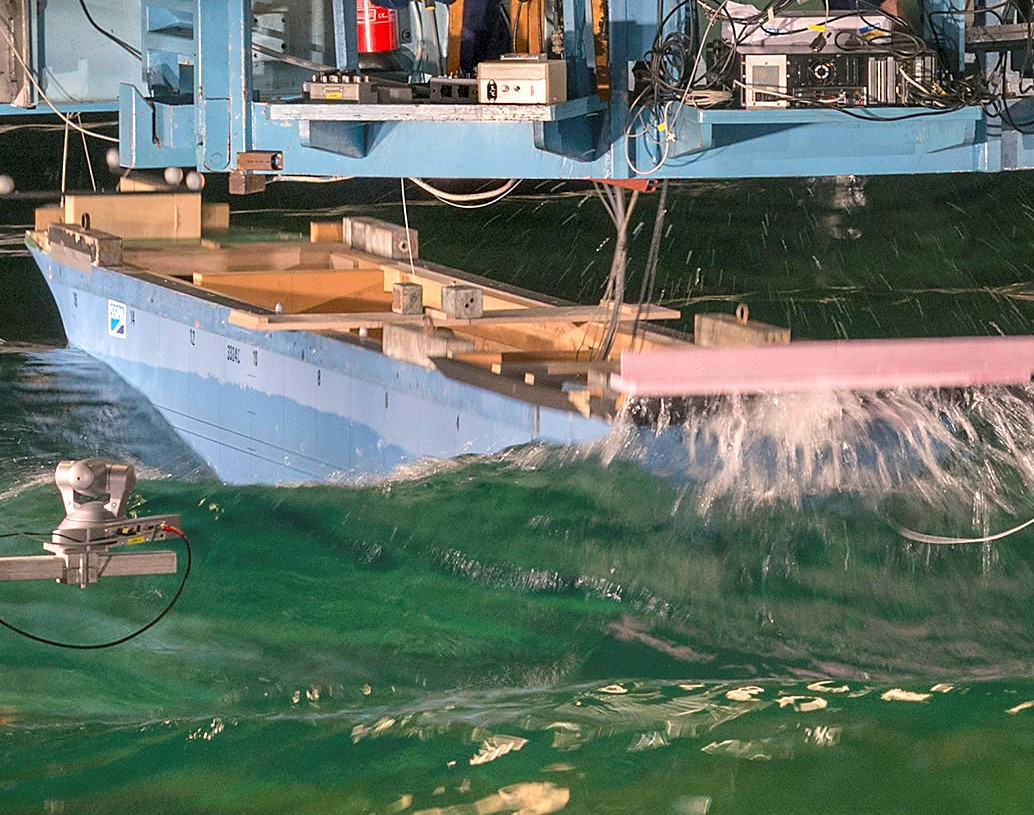
\includegraphics[width=\textwidth]{kappa/images/seakeeping.jpg}
         \caption{Seakeeping}
         \label{fig:seakeeping}
     \end{subfigure}
     \hfill
     \begin{subfigure}[b]{0.45\textwidth}
         \centering
         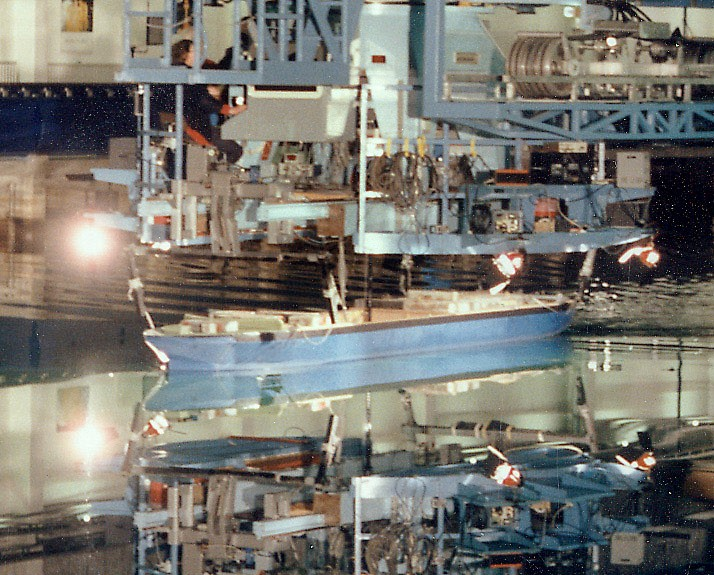
\includegraphics[width=\textwidth]{kappa/images/manoeuvring.jpg}
         \caption{Manoeuvring}
         \label{fig:manoeuvring}
     \end{subfigure}
     \hfill
    \caption{Seakeeping and manoeuvring model tests, copyright SSPA Sweden AB}
    \label{fig:seakeeping_and_manoeuvring}

\end{figure}

The background of modelling the SDTs with white-, black- or grey-box models is first introduced in this chapter followed by a brief literature review. The motivation and objective of this research is then stated followed by assumptions and limitations.

\section{Background}
Shipbuilding 4.0, at the principles of the Industry 4.0, will transform the design, manufacturing, operation, shipping, services, production systems, maintenance and value chains in all aspects of the shipbuilding 
industry \cite{stanic_toward_2018}.
The emergence of Internet-of-Things (IoT) has led to the introduction of the Internet-of-Ships (IoS) paradigm. \begin{quote} IoS is the interconnecting of sensing objects, such as ships, crews, cargoes, onboard equipments, waterway environment, waterway facilities, shore-based facilities, and other navigation elements, which are embedded with a variety of sensor and heterogeneous network technologies to enable these objects to collect and exchange data \cite{liu_internet_2016-1}.\end{quote}
Safety enhancements, route planning and optimization, energy efficiency, automatic berthing and autonomous shipping are some of the emerging applications for the IoS \cite{aslam_internet_2020}.
A SDT as a digital copy of a real ship, is one approach to achieve this \cite{chen_review_2021}. 
SDTs are data-driven in contrast to the related term Virtual Prototyping (VP), which is instead model based \cite{major_framework_2021}. A SDT is generally a model for an existing ship from where data can be collected and the VPs are generally prototypes for future ships, where no operational data is yet available.

The models for VP and SDT can generally be categorized as white-, black- or grey-box models. Where 
white-box models are used in VP and either black-box or grey-box models are used in the SDTs. 
\begin{itemize}
    \item White-box modeling \\
    involves applying physical principles, so that no observed data is required, for instance Computational Fluid Dynamics (CFD). Semi-empirical models where unknown physical constants have been derived from historical experiments, can also be considered as white-box models \cite{leifsson_grey-box_2008}.  

    \item Black-box modeling \\
    means that parameters do not have physical significance but where the objectives is to find a good model that fits the observed data \cite{lindskog_tools_1995}.
    
    \item Grey-box modeling \\
    is a combination of white-box and black-box modeling methods, so that both a physical model and data is used. This concept is also referred as semi-physical modeling, hybrid modeling or semi-mechanistic modeling in the literature \cite{leifsson_grey-box_2008}. 
\end{itemize}

\noindent In a grey box model the white and black parts can be combined in several ways using either a serial or parallel approach \cite{leifsson_grey-box_2008} as seen in Fig.\ref{fig:greycombinations}. 

\begin{figure}[H]
    \centering
    \begin{subfigure}[b]{0.3\textwidth}
    \centering
    \begin{tikzpicture}[node distance=2cm]
    \node (white-box) [white-box] {White-box};
    \node (black-box) [black-box, right of=white-box, xshift=2cm] {Black-box};
    \draw [arrow] (white-box) -- (black-box);
    \end{tikzpicture}
    \caption{Serial grey-box}
    \label{fig:serial1}
    \end{subfigure}

    
    \begin{subfigure}[b]{0.3\textwidth}
    \centering
    \begin{tikzpicture}[node distance=2cm]
    \node (black-box) [black-box] {Black-box};
    \node (white-box) [white-box, right of=black-box, xshift=2cm] {White-box};
    \draw [arrow] (black-box) -- (white-box);
    \end{tikzpicture}
    \caption{Serial grey-box}
    \label{fig:serial2}
    \end{subfigure}

    \begin{subfigure}[b]{0.3\textwidth}
    \centering
    \begin{tikzpicture}[node distance=2cm]
    \node (black-box) [black-box] {Black-box};
    \node (white-box) [white-box, below of=black-box] {White-box};
    \node (join) [process, right of=black-box, xshift=2cm, yshift=-1cm] {join};
    \draw [arrow] (black-box) -- (join);
    \draw [arrow] (white-box) -- (join);
    \end{tikzpicture}
    \caption{Parallel grey-box}
    \label{fig:parallel}
    \end{subfigure}
    \caption{Several ways to combine white- and black-box models in grey box models.}
    \label{fig:greycombinations}
\end{figure}

\section{Literature review}
Ship digital twin (SDT) has a a positive trend in the number of publications during the recent years (2018-2021)  \cite{assani_ships_2022}. Most of the papers concerns ship equipment such as electric power systems, propulsion system, ship hull structure and marine diesel engines \cite{assani_ships_2022}. Only a minor part of the SDT applications handle ship trajectory, speed and fuel consumption \cite{assani_ships_2022}.   
Even though SDT is not explicitly mentioned, there are a lot of papers published about methods that can be used as SDTs. \cite{lang_comparison_2022} predicted the propulsion power for a chemical tanker for three test case voyages with high accuracy, using ML black-box modeling. The manoeuvres where however excluded. In another paper \cite{nielsen_machine_2022} used grey-box modelling for manoeuvring prediction of a ferry where a deep learning model (black-box) captures the residues between first-principles model (white-box) and observed data. These are very promising works that also show that there is still a lot to be done withing the field. 

Some of the publications within system identification of the ship's manoeuvring dynamics are summarized in \autoref{tab:references} categorized as black-box or grey-box models.
\begin{savenotes}\sphinxattablestart
\centering
\sphinxcapstartof{table}
\sphinxthecaptionisattop
\sphinxcaption{System identification references}\label{\detokenize{00.02_introduction:tab-methods}}
\sphinxaftertopcaption
\begin{tabulary}{\linewidth}[t]{|T|T|T|T|T|}
\hline
\sphinxstyletheadfamily 
\sphinxAtStartPar
Method
&\sphinxstyletheadfamily 
\sphinxAtStartPar
BB
&\sphinxstyletheadfamily 
\sphinxAtStartPar
GB
&\sphinxstyletheadfamily 
\sphinxAtStartPar
Data
&\sphinxstyletheadfamily 
\sphinxAtStartPar
Reference
\\
\hline
\sphinxAtStartPar
Constrained Least Squares
&
\sphinxAtStartPar
x
&&
\sphinxAtStartPar
model test, CFD
&
\sphinxAtStartPar
\cite{araki_estimating_2012}
\\
\hline
\sphinxAtStartPar
Neural network
&
\sphinxAtStartPar
x
&&
\sphinxAtStartPar
model test
&
\sphinxAtStartPar
\cite{he_nonparametric_2022}
\\
\hline
\sphinxAtStartPar
Gaussian process
&
\sphinxAtStartPar
x
&&
\sphinxAtStartPar
model test
&
\sphinxAtStartPar
\cite{xue_identification_2021}
\\
\hline
\sphinxAtStartPar
Kalman filter maximum likelihood
&&
\sphinxAtStartPar
x
&
\sphinxAtStartPar
full scale
&
\sphinxAtStartPar
\cite{astrom_identification_1976}
\\
\hline
\sphinxAtStartPar
Unscented kalman filter
&&
\sphinxAtStartPar
x
&
\sphinxAtStartPar
full scale
&
\sphinxAtStartPar
\cite{revestido_herrero_two-step_2012}
\\
\hline
\sphinxAtStartPar
Extended kalman filter
&&
\sphinxAtStartPar
x
&
\sphinxAtStartPar
full scale
&
\sphinxAtStartPar
\cite{perera_system_2015}
\\
\hline
\sphinxAtStartPar
Extended kalman filter
&&
\sphinxAtStartPar
x
&
\sphinxAtStartPar
simulated
&
\sphinxAtStartPar
\cite{shi_identification_2009}
\\
\hline
\sphinxAtStartPar
SVR
&&
\sphinxAtStartPar
x
&
\sphinxAtStartPar
simulated
&
\sphinxAtStartPar
\cite{zhu_parameter_2017}, \cite{wang_parameter_2021}
\\
\hline
\sphinxAtStartPar
SVR
&&
\sphinxAtStartPar
x
&
\sphinxAtStartPar
model test
&
\sphinxAtStartPar
\cite{luo_parameter_2016}
\\
\hline
\sphinxAtStartPar
Genetic algorithm
&&
\sphinxAtStartPar
x
&
\sphinxAtStartPar
lake test
&
\sphinxAtStartPar
\cite{miller_ship_2021}
\\
\hline
\end{tabulary}
\par
\sphinxattableend\end{savenotes} 
\noindent The system identification can be applied on full scale data \cite{astrom_identification_1976}, \cite{perera_system_2015}, \cite{revestido_herrero_two-step_2012} which has the highest uncertainty, both in terms of model uncertainty and measurement uncertainty which is therefore the hardest task, but also the most relevant. The uncertainty can be reduced by instead using model test data as in \cite{araki_estimating_2012}, \cite{he_nonparametric_2022}, \cite{xue_identification_2021}, \cite{miller_ship_2021} and \cite{luo_parameter_2016} . The uncertainty can be further reduced by using simulated data as in \cite{shi_identification_2009}, \cite{zhu_parameter_2017}, \cite{wang_parameter_2021} which can show the potential of new methods with the benefit that the true model is known, but one also has to remember that the objective is to identify real objects, not its mathematical model \cite{miller_ship_2021}.

Black-box modeling was used in \cite{he_nonparametric_2022}, using neural network, and in \cite{xue_identification_2021}, using gaussian process. The nonparametric models are related, where the system structure is known but no parameters are required as seen in \cite{pongduang_nonparametric_2020}. However, most of the system identification methods for ship manoeuvring models use the grey-box modeling by assuming a predefined mathematical model, which reduces the problem to a parameter estimation.
The Kalman Filter (KF) combined with Maximum Likelihood Estimation was proposed already in 1976 \cite{astrom_identification_1976} to develop a linear manoeuvring model based on manually recorded data in 1969 onboard the Atlantic Song freighter. The Extended Kalman Filter (EKF) can also estimate parameters if the parameters are represented as states of the state space model. This technique was used on a nonlinear Nomoto model \cite{perera_system_2015} and a 3 degree of freedom model (3DOF) \cite{shi_identification_2009}. EKF was used in \cite{araki_estimating_2012} with constrained parameters based on physical reasoning and prior knowledge using constrained least squares regression. Unscented Kalman Filter (UKF), which has been proposed as an improvement to the EKF in handling nonlinear systems, was used in \cite{revestido_herrero_two-step_2012}.
Support Vector Regression (SVR) has been investigated in \cite{zhu_parameter_2017}, \cite{wang_parameter_2021} and \cite{luo_parameter_2016}. A genetic algorithm was used in \cite{miller_ship_2021} for the system identification of model test performed on a lake.





%"Critic" to what has been done before
\section{Motivation and objective}
\label{sec:motivation}
% Motivation:
Huge amounts of data concerning ships' operation is collected daily around the oceans. We are still figuring out ways to make use of it. Using SDTs is one way, modelled as white-, black- or grey-boxes.
The black-box modeling is entirely data driven, which means that no prior understanding of the system generating the data is needed and is therefore an attractive option for the SDT modelling. The black-box modeling may however give infeasible models outside the domain covered by the available data \cite{nielsen_machine_2022}. 

The white-box modeling does not have this problem, but does on the other hand require a full understanding of the system, which may be possible for special cases, but in general not possible for the complex scenarios and nonlinearities of a ship operating at sea \cite{miller_ship_2021}. 
In the deep sea: wind, waves and current will add complexity. In coastal areas water depth and bank-effects will also add complexity \cite{nielsen_machine_2022}. 
Also, even if the sea is modelled perfectly, long term predictions are not possible due to the behaviour known as deterministic chaos \cite{lorenz_deterministic_1963}, popularly known as ''butterfly effect'', where only a very small difference in the initial conditions result in totally different outcomes. Two weeks are for instance believed to be the upper limit for weather forecasts  \cite{zhang_what_2019}. Grey-box modelling is therefore used in this thesis, which is an attempt to bridge these problems, to either mitigate the white-box modelling error or the black-box extrapolation error. 

It is often practical to first assume higher levels of simplifications and approximations for the problem under study and thereafter, step by step, increase the complexity of the problem. In this way, the effects of various factors can be initially studied in a rather isolated way. 
Ship rigid body dynamics at full scale sea conditions comprises uncertainties from:
\begin{itemize}
    \item the \textbf{environment}: wind, waves and currents
    \item the \textbf{ship}: geometry and mass properties
    \item the \textbf{measurements}
\end{itemize}

\noindent A simplification made in this thesis, is to limit the uncertainties at full scale sea conditions, by instead using model tests data, from a controlled laboratory environment. A majority of the publications within this field, such as \cite{shi_identification_2009}, \cite{perera_system_2015}, \cite{zhu_parameter_2017}, \cite{wang_parameter_2021} and \cite{xue_hydrodynamic_2020} simplifies this even further by using simulated data, which can be too much of a simplification as we identify real objects, not its mathematical model \cite{miller_ship_2021}.
The main objective with this thesis is therefore to:
% Objective: 
\begin{quote} 
Develop system identification methods for grey box models of ship rigid body dynamics in calm waters. 
\end{quote}

\noindent 
The goals for this thesis, to fulfill the research objective, have been formulated following the step by step approach as described above, with reduced complexity and then gradually increasing the complexity:

\subsubsection*{Roll motion model}
The first goal of the thesis is therefore to develop a model for the calm water ship rigid body dynamics in the roll degree of freedom, based on model test data.

\subsubsection*{Manoeuvring model}
The second goal is to increase the complexity by adding the surge, sway and yaw degrees of freedoms, addressing the manoeuvring problem.

\subsubsection*{Model generalization}
The models must be able to make predictions outside the domain covered by the available data, in order to be of practical use in IoS applications.

\section{Assumptions and limitations}
%Calm waters...
Calm water condition is a simplification of the real sea condition that a ship encounters. This condition assumes that the influences from encountering wind, waves and currents are neglected. These assumptions simplifies the system identification, by reducing the degrees of freedoms to: surge, sway, yaw and roll. 
The rigid body assumption simplifies the ship as a stiff body that does not transform under the act of forces. 
Also note that all result are not necessarily directly transferable to full scale when model scale data is used, considering potential scale effects. 

\section{Outline of the thesis}
Chapter \ref{ch:models} presents the models for ship rigid body dynamics used in this thesis. The models for roll motion is introduced in Section \ref{sec:roll} and the manoeuvring motion models are introduced in Section \ref{sec:manoeuvring model}. These models represent the physical principles and thereby the white-box part of the developed grey-box models.
Parameter estimations, representing the black-box part, are used to regress the parameters of the white-box models. The parameter estimations are introduced in Chapter \ref{ch:methods} for the roll motion and the manoeuvring motion in Section \ref{sec:_roll} and Section \ref{sec:_VMM}. 
A short summary of the appended papers, including research activities and a selection of the important results is presented in chapter \ref{ch:results}, followed by the conclusions in chapter \ref{ch:conclusions} and plans for future work in chapter \ref{ch:future_work}.